\documentclass[border=10pt]{standalone}
\usepackage{tikz}
\usetikzlibrary{arrows.meta, positioning, fit, backgrounds, calc}
\usepackage[T1]{fontenc}
\usepackage{helvet}
\renewcommand{\familydefault}{\sfdefault}

\definecolor{darkblue}{RGB}{0, 0, 139}
\definecolor{pinkdash}{RGB}{255, 50, 120}

\begin{document}
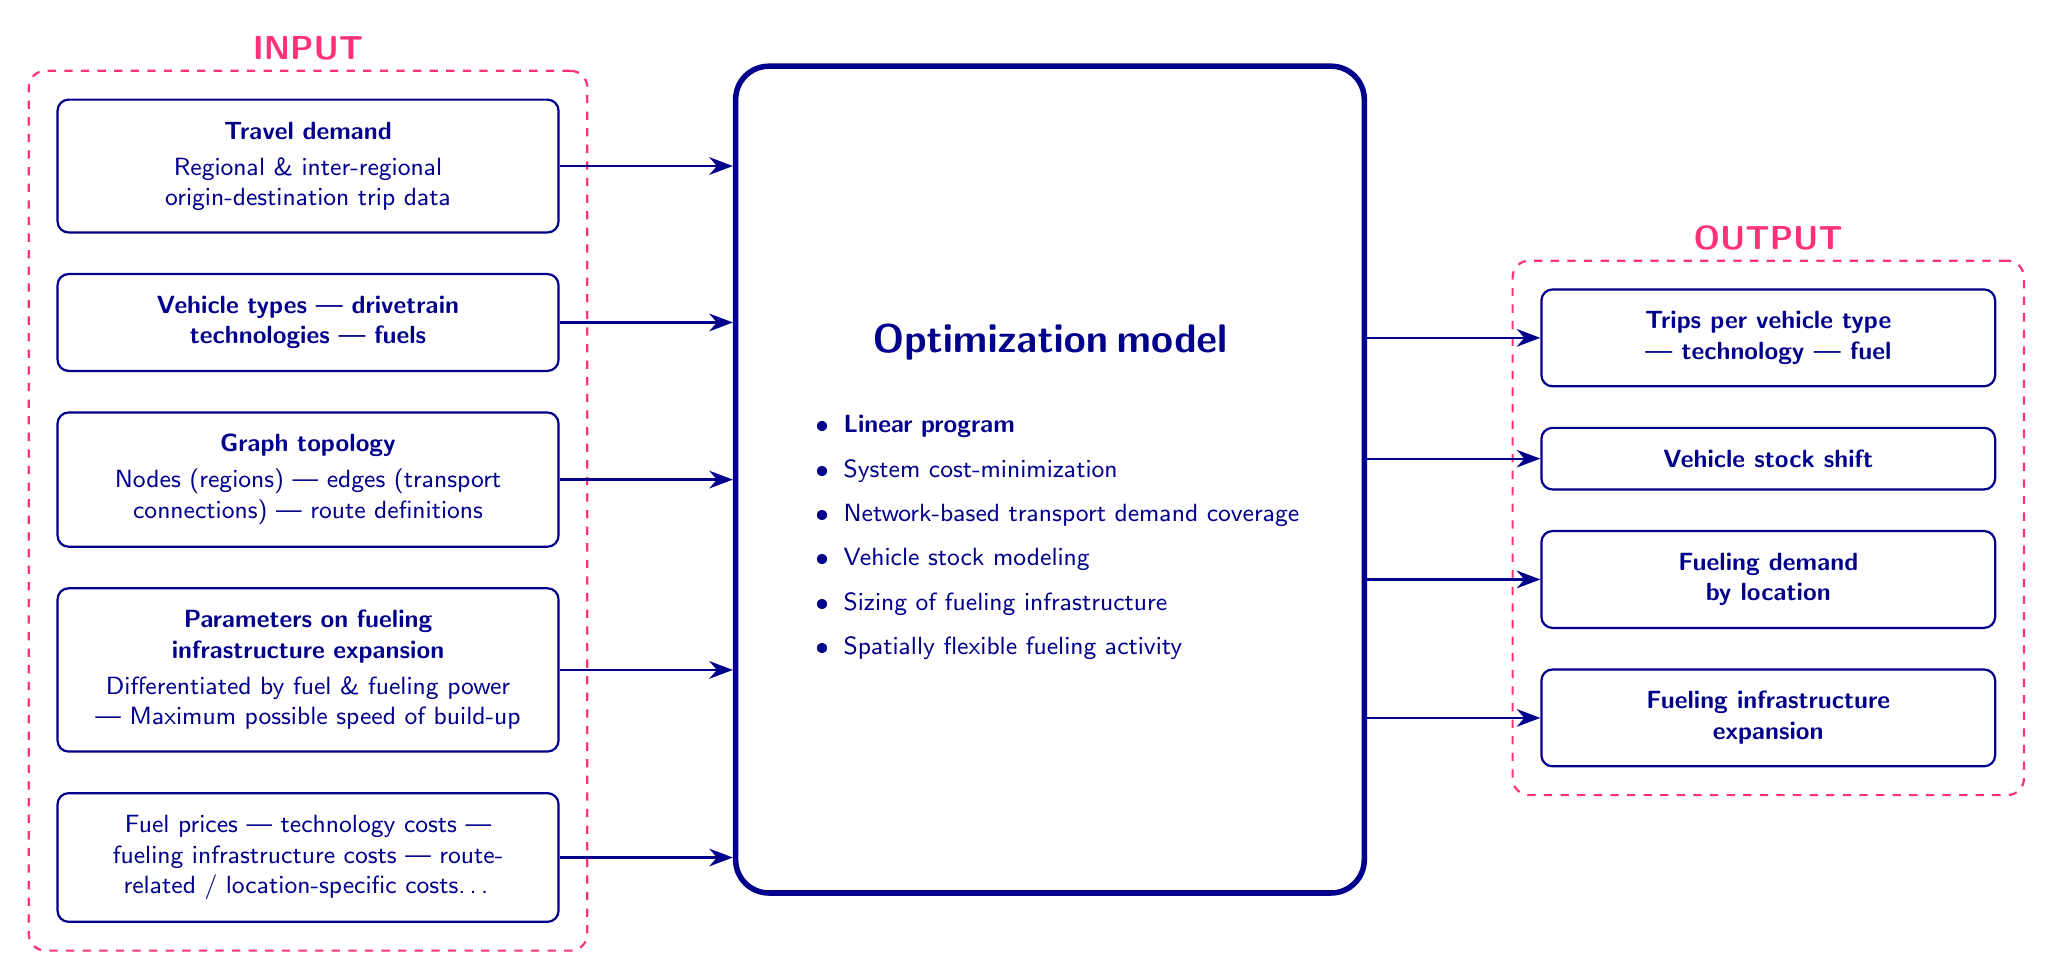
\begin{tikzpicture}[
    node distance=0.5cm,
    inputbox/.style={
        draw=darkblue, thick, rounded corners=4pt,
        text width=5.8cm, align=center, inner sep=8pt,
        font=\small, text=darkblue
    },
    outputbox/.style={
        draw=darkblue, thick, rounded corners=4pt,
        text width=5.2cm, align=center, inner sep=8pt,
        font=\small\bfseries, text=darkblue
    },
    modelbox/.style={
        draw=darkblue, line width=2pt, rounded corners=12pt,
        text width=7cm, align=left, inner sep=14pt,
        font=\small, text=darkblue
    },
    arrow/.style={-{Stealth[length=3mm]}, darkblue, thick},
    dashed border/.style={draw=pinkdash, dashed, thick, rounded corners=6pt}
]

% INPUT BOXES
\node[inputbox] (input1) {
    \textbf{Travel demand}\\[2pt]
    Regional \& inter-regional origin-destination trip data
};

\node[inputbox, below=of input1] (input2) {
    \textbf{Vehicle types | drivetrain\\technologies | fuels}
};

\node[inputbox, below=of input2] (input3) {
    \textbf{Graph topology}\\[2pt]
    Nodes (regions) | edges (transport connections) | route definitions
};

\node[inputbox, below=of input3] (input4) {
    \textbf{Parameters on fueling\\infrastructure expansion}\\[2pt]
    Differentiated by fuel \& fueling power | Maximum possible speed of build-up
};

\node[inputbox, below=of input4] (input5) {
    Fuel prices | technology costs | fueling infrastructure costs | route-related / location-specific costs\ldots
};

% MODEL BOX - centered vertically with inputs, tall enough to span all input boxes
\node[modelbox, right=2.2cm of input3, minimum height=10.5cm] (model) {
    \begin{center}\textbf{\Large Optimization model}\end{center}\vspace{4pt}
    \begin{itemize}
        \setlength{\itemsep}{3pt}
        \item \textbf{Linear program}
        \item System cost-minimization
        \item Network-based transport demand coverage
        \item Vehicle stock modeling
        \item Sizing of fueling infrastructure
        \item Spatially flexible fueling activity
    \end{itemize}
};

% OUTPUT BOXES - centered vertically with model
\node[outputbox, right=2.2cm of model, yshift=1.8cm] (output1) {
    Trips per vehicle type\\| technology | fuel
};

\node[outputbox, below=of output1] (output2) {
    Vehicle stock shift
};

\node[outputbox, below=of output2] (output3) {
    Fueling demand\\by location
};

\node[outputbox, below=of output3] (output4) {
    Fueling infrastructure\\expansion
};

% ARROWS: INPUT -> MODEL (horizontal to model west edge)
\draw[arrow] (input1.east) -- (input1.east -| model.west);
\draw[arrow] (input2.east) -- (input2.east -| model.west);
\draw[arrow] (input3.east) -- (model.west);
\draw[arrow] (input4.east) -- (input4.east -| model.west);
\draw[arrow] (input5.east) -- (input5.east -| model.west);

% ARROWS: MODEL -> OUTPUT (horizontal from model east edge)
\draw[arrow] (model.east |- output1.west) -- (output1.west);
\draw[arrow] (model.east |- output2.west) -- (output2.west);
\draw[arrow] (model.east |- output3.west) -- (output3.west);
\draw[arrow] (model.east |- output4.west) -- (output4.west);

% DASHED BORDERS
\begin{scope}[on background layer]
    \node[dashed border, fit=(input1)(input5), inner sep=10pt, label={[text=pinkdash, font=\bfseries\large]above:INPUT}] {};
    \node[dashed border, fit=(output1)(output4), inner sep=10pt, label={[text=pinkdash, font=\bfseries\large]above:OUTPUT}] {};
\end{scope}

\end{tikzpicture}
\end{document}
